\documentclass[english,9pt,aspectraio=169]{beamer}
\usepackage{etex}
\usetheme{uzhneu-en-informal}
%\usepackage{uarial}
\usepackage[T1]{fontenc}
\usepackage[utf8]{inputenc}
\RequirePackage{graphicx,ae}
\usepackage{bm}
\usepackage{fancybox,amssymb,color}
\usepackage{pgfpages}
\usepackage{booktabs}
\usepackage{verbatim}
\usepackage{animate}
\usepackage{numprint}
\usepackage{dsfont}
\usepackage{tikz}
\usepackage{amsmath,natbib}
\usepackage{mathbbol}
\usepackage{babel}
\usepackage{SweaveSlides}
\usepackage{multicol}
\usepackage{xcolor}


\usetheme{uzhneu-en-informal}
\DeclareMathOperator{\po}{Poisson}
\DeclareMathOperator{\G}{Gamma}
\DeclareMathOperator{\Be}{Beta}
\DeclareMathOperator{\logit}{logit}
\def\n{\mathop{\mathcal N}}

\definecolor{Gray}{RGB}{139,137,137}
\definecolor{darkred}{rgb}{0.8,0,0}
\definecolor{Green}{rgb}{0,0.8,0.3}
\definecolor{Blue}{rgb}{0,0,1}
\def\myalert{\textcolor{darkred}}
\def\myref{\textcolor{Gray}}
\setbeamercovered{invisible}

\renewcommand{\baselinestretch}{1.2}
\beamertemplateballitem
\DeclareMathOperator{\cn}{cn} % Copy number
\DeclareMathOperator{\ccn}{ccn} % common copy number
\DeclareMathOperator{\p}{p} % common copy number
\DeclareMathOperator{\E}{E} % common copy number
\DeclareMathOperator{\given}{|} % common copy number
\def\given{\,|\,}
\def\na{\tt{NA}}
\def\nin{\noindent}
\pdfpageattr{/Group <</S /Transparency /I true /CS /DeviceRGB>>}
\def\eps{\varepsilon}

\renewcommand{\P}{\operatorname{\mathsf{Pr}}} % Wahrscheinlichkeitsmaß
\def\eps{\varepsilon}
\def\logit{\text{logit}}
%\newcommand{\E}{\mathsf{E}} % Erwartungswert
\newcommand{\Var}{\text{Var}} % Varianz
\newcommand{\NBin}{\text{NBin}}
\newcommand{\Po}{\text{Po}}
\newcommand{\N}{\mathsf{N}}

\newcommand{\ball}[1]{\begin{pgfpicture}{-1ex}{-0.65ex}{1ex}{1ex}
\usebeamercolor[fg]{item projected}

{\pgftransformscale{1.75}\pgftext{\normalsize\pgfuseshading{bigsphere}}}
{\pgftransformshift{\pgfpoint{0pt}{0.5pt}}
\pgftext{\usebeamerfont*{item projected}{#1}}}
\end{pgfpicture}}%
\usepackage{multicol}
\newcommand{\ballsmall}[1]{\begin{pgfpicture}{-1ex}{-0.65ex}{.2ex}{.2ex}

{\pgftransformscale{1}\pgftext{\normalsize\pgfuseshading{bigsphere}}}
{\pgftransformshift{\pgfpoint{0pt}{0.5pt}}
\pgftext{\usebeamerfont*{item projected}{#1}}}
\end{pgfpicture}}%




\begin{document}


\fboxsep5pt

\frame{
\title[]{ \centering \Huge Kurs Bio144: \\
Datenanalyse in der Biologie}%\\[.3cm]
\author[Stefanie Muff, Owen L.\ Petchey]{\centering Stefanie Muff  \& Owen L.\ Petchey }
%\institute[]{Institute of Social and Preventive Medicine \\ Institute of Evolutionary Biology and Environmental Studies}
\date[]{Week 3: Multiple linear regression \\ 9./10. March 2017}


\maketitle
}


\frame{\frametitle{Overview (todo: check)}
\begin{itemize}

\item Checking the assumptions of linear regression
\item Tukey-Anscombe diagram, QQ-plot 
\item Multiple predictors $x_1$, $x_2$, \ldots, $x_p$
\item $R^2$ in multiple linear regression
\item $t$-tests, $F$-tests and $p$-values
\item Binary and factor covariates

\end{itemize}
}



\frame{\frametitle{Course material covered today}
\begin{itemize}
\item Chapters 3.1, 3.2a-q of \emph{Lineare Regression}
\item Chapters 4.1 4.2f, 4.3a-e of \emph{Lineare Regression}
\item Chapter 11.2 in \emph{Statistische Datenanalyse}
\end{itemize}
}

\frame[containsverbatim]{\frametitle{Recap of last week I}

\begin{itemize}
\item The linear regression model for the data $\bm{y}=(y_1,\ldots,y_n)$ given $\bm{x}=(x_1,\ldots,x_n)$ is
$$y_i = \alpha + \beta x_i + e_i \ , \qquad e_i \sim \N(0,\sigma_e^2) \  \text{independent}.$$\\[2mm]
\item Estimate the parameters $\alpha$, $\beta$ and $\sigma_e^2$ by least squares.\\[2mm]
\item The estimated parameters $\hat\alpha$, $\hat\beta$ contain \myalert{uncertainty} and are normally distributed around the true values. %(actually, also $\hat\sigma_e^2$...). \\[2mm]
\item Use the knowledge about the distribution to formulate \myalert{statistical tests}, such as: Is $\beta=0$?\\[2mm]
\item All this is done automatically by R:\\[2mm]
\begin{Schunk}
\begin{Sinput}
> summary(r.bodyfat)$coef
\end{Sinput}
\begin{Soutput}
              Estimate Std. Error   t value     Pr(>|t|)
(Intercept) -26.984368  2.7689004 -9.745518 3.921511e-19
bmi           1.818778  0.1083411 16.787522 2.063854e-42
\end{Soutput}
\end{Schunk}
\end{itemize}

}


\frame[containsverbatim]{\frametitle{Recap of last week II}

\begin{itemize}
\item Confidence and prediction ranges:
\end{itemize}
\begin{center}
\setkeys{Gin}{width=0.65\textwidth}
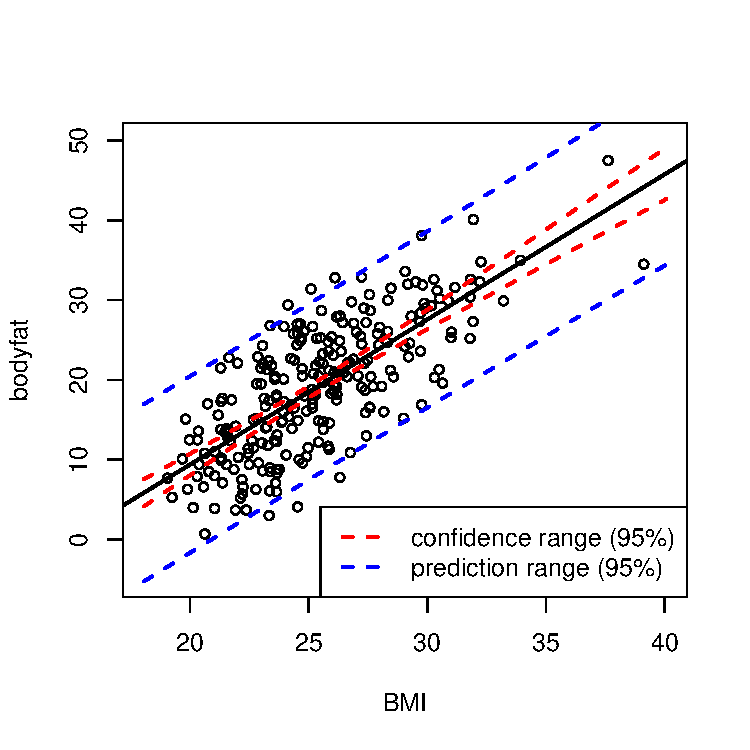
\includegraphics{Bio144_2017_week3-confpred}
\end{center}
}


\frame[containsverbatim]{\frametitle{Recap of last week III}
Remember: 
The assumption in linear regression is that the residuals follow a $\N(0,\sigma_e^2)$ distribution, implying that :\\[2mm]
\colorbox{lightgray}{\begin{minipage}{10cm}
\begin{enumerate}[a)]
\item The expected value of $e_i$ is 0: $\E(e_i)=0$.\\[2mm]
\item All $e_i$ have the same variance: $\Var(e_i)=\sigma_e^2$. \\[2mm]
\item The $e_i$ are normally distributed.\\[2mm]
\item The $e_i$ are independent of each other.
\end{enumerate}
\end{minipage}}
~\\
We started to do some residual analysis using the \myalert{Tukey-Anscombe plot} and the \myalert{Histogram} of the residuals $R_i$.\\[-4mm]

\begin{center}
\setkeys{Gin}{width=0.6\textwidth}
\includegraphics{Bio144_2017_week3-MCs}
\end{center}

}

\frame[containsverbatim]{\frametitle{Another useful diagnostic plot: The QQ-plot}
Usually, not the histogram of the residuals is plotted, but the so-called \myalert{quantile-quantile} (QQ) plot. The quantiles of the observed distribution are plotted against the quantiles of the respective theoretical (normal) distribution:

\begin{multicols}{2}
\setkeys{Gin}{width=0.4\textwidth}
\begin{Schunk}
\begin{Sinput}
> qqnorm(r.bodyfat$residuals)
> qqline(r.bodyfat$residuals)
\end{Sinput}
\end{Schunk}
\includegraphics{Bio144_2017_week3-QQ1}
\\
If the points lie approximately on a straight line, the data is fairly normally distributed.\\[2mm]

This is often ``tested'' by eye, and needs some experience.
\end{multicols}
}

\frame[containsverbatim]{

Please read ``Quantil-Quantil-Diagramme'', Chapter 11.2., p.258-261, in ``Statistische Datenenalyse'' by W. Stahel (Mat183 literature).\\[2mm]

It gives a very nice and intuitive description of QQ diagrams! \\

\setkeys{Gin}{width=0.8\textwidth}
\includegraphics{Bio144_2017_week3-006}
~\\
The idea is that, for each observed point, theoretical quantiles are plotted against the sample quantiles.
}

\frame{
\begin{center}
{\Large\textcolor{blue}{Multiple linear regression}}
\end{center}
}

\frame[containsverbatim]{\frametitle{Bodyfat example}
We have so far modelled bodyfat in dependence of bmi, that is: $(body fat)_i = \alpha + \beta \cdot bmi_i + e_i$.\\[2mm]

However, other predictors might also be relevant for an accurate prediction of bodyfat.\\[4mm]

{\bf Examples:} Age, neck fat (Nackenfalte), hip circumference, abdomen circumference etc.
\begin{center}
\setkeys{Gin}{width=1\textwidth}
\includegraphics{Bio144_2017_week3-007}
\end{center}

}

\frame[containsverbatim]{
Or again the pairs plot:
\setkeys{Gin}{width=0.8\textwidth}
\begin{Schunk}
\begin{Sinput}
> pairs(d.bodyfat)
\end{Sinput}
\end{Schunk}
\includegraphics{Bio144_2017_week3-008}
}

\frame[containsverbatim]{\frametitle{Multiple linear regression model}
The idea is simple: just {\bf extend the linear model by additional predictors}.\\[4mm]

\begin{itemize}
\item Given several influence factors $x_i^{(1)}$, \ldots, $x_i^{(m)}$, 
the straightforward extension of the simple linear model is\\[4mm]

\colorbox{lightgray}{\begin{minipage}{10cm}
\begin{eqnarray*}
y_i &=& \beta_0 + \beta_1 x_i^{(1)} + \beta_2 x_i^{(2)} + \ldots + \beta_2 x_i^{(m)} + e_i  \\[2mm]
\text{with  } \ e_i &\sim& \N (0,\sigma_e^2).
\end{eqnarray*}
\end{minipage}}
~\\[6mm]
\item The parameters of this model are $\bm\beta=(\beta_0,\beta_1,\ldots,\beta_m)$ and $\sigma_e^2$.
\end{itemize}
}

\frame{\frametitle{}
The components of $\bm\beta$ are again estimated using the {\bf least squares} method. Basically, the idea is (again) to minimize 
$$\sum_{i=1}^n r_i^2$$
with 
$$r_i = y_i - (\beta_0 + \beta_1 x_i^{(1)} + \beta_2 x_i^{(2)} + \ldots + \beta_2 x_i^{(m)}) $$ 

It is a bit more complicated than for simple linear regression, see Sections 3.3 and 3.4 of the Stahel script. \\[4mm]

Some {\bf linear algebra} is needed to understand these sections, but we do not look into this for the moment. (It will come later in week 6.) \\[4mm]


}

\frame{\frametitle{Multiple linear regression for bodyfat}
Let us regress the proportion (\%) of bodyfat (from last week) on the predictors {\bf bmi} and {\bf age} simultaneously. The model thus is given as\\[4mm]
\begin{eqnarray*}
(bodyfat)_i &=& \beta_0 + \beta_1 \cdot bmi_i + \beta_2 \cdot age_i + e_i \ , \\
\text{with} \quad e_i &\sim& \N(0,\sigma_e^2) \ .
\end{eqnarray*}
}

\frame[containsverbatim]{\frametitle{}
\emph{Before} we estimate the parameters, let us ask the questions that we intend to answer:\\[6mm]
\begin{enumerate}
\item Does the {\bf ensemble} of all covariates explain a relevant part of the variability of the response?\\[4mm]
\item If yes, which influence variables are good predictors of bodyfat? \\[4mm]
\item How good is the overall model fit?
\end{enumerate}

}


\frame[containsverbatim]{\frametitle{Multiple linear regression with R}
\vspace{-8mm}
Let's now fit the model with R, and quickly glance at the output:\\[4mm]

\begin{Schunk}
\begin{Sinput}
> r.bodyfatM <- lm(bodyfat ~ bmi + age ,d.bodyfat) 
\end{Sinput}
\end{Schunk}
\begin{Schunk}
\begin{Sinput}
> summary(r.bodyfatM)
\end{Sinput}
\begin{Soutput}
Call:
lm(formula = bodyfat ~ bmi + age, data = d.bodyfat)

Residuals:
     Min       1Q   Median       3Q      Max 
-12.0415  -3.8725  -0.1237   3.9193  12.6599 

Coefficients:
             Estimate Std. Error t value Pr(>|t|)    
(Intercept) -31.25451    2.78973 -11.203  < 2e-16 ***
bmi           1.75257    0.10449  16.773  < 2e-16 ***
age           0.13268    0.02732   4.857 2.15e-06 ***
---
Signif. codes:  0 ‘***’ 0.001 ‘**’ 0.01 ‘*’ 0.05 ‘.’ 0.1 ‘ ’ 1

Residual standard error: 5.329 on 240 degrees of freedom
Multiple R-squared:  0.5803,	Adjusted R-squared:  0.5768 
F-statistic: 165.9 on 2 and 240 DF,  p-value: < 2.2e-16
\end{Soutput}
\end{Schunk}
}

\frame[containsverbatim]{\frametitle{Model checking}
Before we look at the results, we have to check if the modelling assumptions are fulfilled:
\begin{center}
\setkeys{Gin}{width=0.9\textwidth}
\includegraphics{Bio144_2017_week3-modelChecks}
\end{center}

This seems ok, so continue with answering questions 1-3.
}



\frame[containsverbatim]{\frametitle{Question 1: Does the model have some explanatory power?}
To answer question 1, we need to perform a so-called $F$-test. The results of the test are displayed in the final line of the regression summary. Here, it says:\\[2mm]

\texttt{F-statistic: 165.9 on 2 and 240 DF, p-value: < 2.2e-16} \\[2mm]

So apparently (and we already suspected that) the model has some explanatory power.\\[8mm]

\scriptsize{
*The $F$-statistic and -test is briefly recaptured in 3.1.f) of the Stahel script, but see also Mat183 chapter 6.2.5. It uses the fact that
%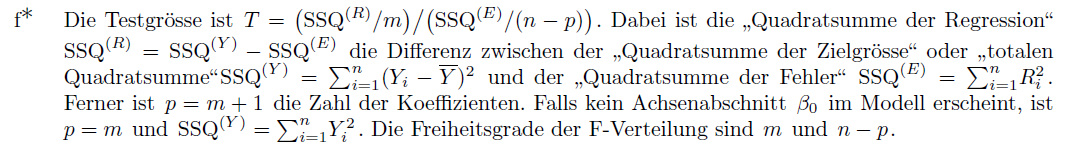
\includegraphics[width=11cm]{pictures/fstar.jpg}
\begin{equation*}
\frac{SSQ^{(R)}/m}{SSQ^{(E)}/(n-p)} \sim F_{m,n-p}
\end{equation*}
follows an $F$-distribution (\texttt{df()} in R) with $m$ and $(n-p)$ degrees of freedom, where $m$ are the number of variables, $n$ the number of data points, $p$ the number of $\beta$-parameters (typically $m+1$). $SSQ^{(E)}=\sum_{i=1}^nR_i^2$ is the squared sum of the residuals, and $SSQ^{(R)} = SSQ^{(Y)} - SSQ^{(E)}$ with $SSQ^{(y)}=\sum_{i=1}^n(y_i-\overline{y})^2$.
}

}

\frame[containsverbatim]{\frametitle{Question 2: Which variables influence the response?}
%' <<summary.bf,results=tex,echo=F>>= 
%' tableRegression(r.bodyfatM)
%' @

\begin{Schunk}
\begin{Sinput}
> summary(r.bodyfatM)$coef
\end{Sinput}
\begin{Soutput}
               Estimate Std. Error    t value     Pr(>|t|)
(Intercept) -31.2545057 2.78973238 -11.203406 1.039096e-23
bmi           1.7525705 0.10448723  16.773060 2.600646e-42
age           0.1326767 0.02731582   4.857137 2.149482e-06
\end{Soutput}
\end{Schunk}
~\\[2mm]

To answer this question, again look at the $t$-tests, for which the $p$-values are given in the final column. Each $p$-value refers to the test for the null hypothesis $ \beta^{(j)}_0=0$ for covariate $x^{(j)}$.\\[2mm]

As in simple linear regression, the $T$-statistic for the $j$-th covariate is calculated as 
%
\begin{equation}\label{eq:beta}
T_j =\frac{\hat\beta_j - {\beta_j}_0}{se^{(\beta_j)}}  \quad\underbrace{=}_{if  {\beta_j}_0=0} \quad  \frac{\hat\beta_j}{se^{(\beta_j)}}\ ,
\end{equation}
with  $se^{(\beta_j)}$ given in the second column of the regression output.\\[2mm]
The distribution of this statistic is $T_j \sim t_{n-p}$. 


}

\frame[containsverbatim]{

Therefore:  A ``small'' $p$-value indicates that the variable is relevant in the model.\\[2mm]

Here, we have 
\begin{itemize}
\item $p<0.001$ for bmi
\item $p<0.001$ for age
\end{itemize}

Thus both, bmi and age seem to have some predictive power for bodyfat. \\[2mm]

Again, a 95\% CI for $\beta_j$ can be calculated with $[\hat\beta - c \cdot \sigma^{(\beta)} ; \hat\beta + c \cdot \sigma^{(\beta)}]$, where $c$ is the 97.5\% quantile of the $t$-distribution with $n-p$ degrees of freedom  (compare to slide 38 of last week). With R:\\[2mm]

\begin{Schunk}
\begin{Sinput}
> confint(r.bodyfatM)
\end{Sinput}
\begin{Soutput}
                  2.5 %      97.5 %
(Intercept) -36.7499929 -25.7590185
bmi           1.5467413   1.9583996
age           0.0788673   0.1864861
\end{Soutput}
\end{Schunk}

}

\frame[containsverbatim]{\frametitle{}
{\bf !However!: }\\[2mm]

The $p$-value and $T$-statistics should only be used as a {\bf rough guide} for the ``significance'' of the coefficients.\\[2mm]

For illustration, let us extend the model a bit more, including also neck, hip and abdomen:\\[4mm]

\begin{Schunk}
\begin{Sinput}
> r.bodyfatM2 <- lm(bodyfat ~ bmi + age + neck + hip + abdomen,d.bodyfat)
> summary(r.bodyfatM2)$coef
\end{Sinput}
\begin{Soutput}
               Estimate Std. Error    t value     Pr(>|t|)
(Intercept) -7.74964673 7.29830233 -1.0618424 2.893881e-01
bmi          0.42647368 0.23132902  1.8435805 6.649276e-02
age          0.01457356 0.02782994  0.5236649 6.010010e-01
neck        -0.80206081 0.19096606 -4.2000177 3.779800e-05
hip         -0.31764315 0.10751209 -2.9544876 3.447492e-03
abdomen      0.83909391 0.08417902  9.9679702 9.035870e-20
\end{Soutput}
\end{Schunk}
~\\[3mm]
It is now much \myalert{less clear what the influences of age ($p=0.60$) and bmi ($p=0.06$) are}. \\[2mm]


}


\frame[containsverbatim]{\frametitle{ }

Basically, the problem is that the variables in the model are correlated and therefore explain similar aspects of \% bodyfat. \\[6mm]


\colorbox{lightgray}{\begin{minipage}{10cm}
This problem is at the heart of many confusions of regression analysis, and we will talk about such issues later in the course.
\end{minipage}}




}

\frame[containsverbatim]{\frametitle{Question 3: How good is the overall model fit?}
To answer this question, we can look at the \myalert{multiple $R^2$} (see Stahel 3.1.h). It is a generalized version of $R^2$ for simple linear regression:\\[2mm]

\colorbox{lightgray}{\begin{minipage}{10cm}
$R^2$ {\bf for multiple linear regression} is defined as the squared correlation between $(y_1,\ldots,y_n)$ and $(\hat{y}_1,\ldots,\hat{y}_n)$, where the $\hat y$ are the fitted values 
\begin{equation*}
\hat{y}_i = \hat\beta_0 + \hat\beta_1 x^{(1)} + \ldots + \hat\beta_m x^{(m)}
\end{equation*}
\end{minipage}}
\vspace{-5mm}
\begin{center}
\setkeys{Gin}{width=0.5\textwidth}
\includegraphics{Bio144_2017_week3-016}
\end{center}
}


\frame{
$R^2$ is also called the \emph{coefficient of determination} or \myalert{``Bestimmtheitsmass''}, because it measures the proportion of the reponse's variability that is explained by the ensemble of all covariates:\\[4mm]

\colorbox{lightgray}{\begin{minipage}{10cm}
\begin{equation*}
R^2 = SSQ^{(R)} / SSQ^{(Y)} = 1 - SSQ^{(E)}/ SSQ^{(Y)}
\end{equation*}
\end{minipage}}
~~\\
Remembering that \\
\begin{eqnarray*}
\text{total variability} &=&  \text{explained variability} + \text{residual variability} \\[2mm]
\sum_{i=1}^n (y_i - \overline{y})^2 &=&  \sum_{i=1}^n (\hat{y_i}-\overline{y})^2 \qquad \quad + \quad \qquad \sum_{i=1}^n (\hat{y_i}-y_i)^2 \\[2mm]
SSQ^{(Y)} &=& SSQ^{(R)} \qquad\qquad \quad + \qquad\quad\qquad SSQ^{(E)} \\[2mm]
\end{eqnarray*}

}

\frame[containsverbatim]{

\begin{center}
\setkeys{Gin}{width=0.6\textwidth}
\includegraphics{Bio144_2017_week3-017}
\end{center}
}


\frame[containsverbatim]{
Let us look at the $R^2$s from the three bodyfat models \\
(model 1: $y\sim bmi$\\
model 2: $y\sim bmi + age$\\
model 3: $y\sim bmi + age + neck + hip + abdomen$):\\[4mm]

\begin{Schunk}
\begin{Soutput}
[1] 0.5390391
\end{Soutput}
\begin{Soutput}
[1] 0.5802956
\end{Soutput}
\begin{Soutput}
[1] 0.718497
\end{Soutput}
\end{Schunk}
 ~\\[2mm]
The models thus explain  $54$ \%, $58$ \% and $72$ \% of the total variability of $y$.\\[5mm]

It thus \emph{seems} that larger models are ``better''. However, $R^2$ does always increase when new variables are included, but this does not mean that the model is more reasonable. \\[2mm]

\myalert{Model selection} is a topic that will be treated in more detail later in this course.
}

\frame{\frametitle{Adjusted $R^2$}
When the sample size $n$ is small with respect to the number of variables $m$ included in the model, an \myalert{adjusted} $R^2$ gives a better (or ``fairer'', i.e.\ unbiased) estimation of the actual variability that is explained by the covariates:

\begin{equation*}
R^2_a = 1-(1-R^2 )\frac{n-1}{n-m-1}
\end{equation*}
~\\
Why $R^2_a$? Todo: explain briefly 
}


\frame[containsverbatim]{\frametitle{Interpretation of the coefficients}
Apart from model checking and thinking about questions 1-3, it is probably even {\bf more important to understand what you \emph{see}.} Look at the output and ask yourself:\\[2mm]

\begin{quote}
What does the regression output actually \emph{mean}?
\end{quote}

% latex table generated in R 3.3.1 by xtable 1.8-2 package
% Thu Oct 27 11:12:00 2016
\begin{table}[!h]
\centering
\begingroup\footnotesize
\begin{tabular}{rrrr}
  \hline
 & Coefficent & 95\%-confidence interval & $p$-value \\ 
  \hline
Intercept & -31.25 & from -36.75 to -25.76 & $<$ 0.0001 \\ 
  bmi & 1.75 & from 1.55 to 1.96 & $<$ 0.0001 \\ 
  age & 0.13 & from 0.08 to 0.19 & $<$ 0.0001 \\ 
   \hline
\end{tabular}
\endgroup
\caption{Parameter estimates of model 3.} 
\label{tab:m3}
\end{table}
Task in teams: Interpret the coefficients, 95\% CIs and $p$-values.
}

\frame[containsverbatim]{\frametitle{Example: Catheter Data}

Catheter length ($y$) for heart surgeries depending on two characteristic variables $x^{(1)}$ and $x^{(2)}$ of the patients. Aim: estimate $y$ from $x^{(1)}$ and  $x^{(2)}$ ($n=12$). Again look at the data first:

\setkeys{Gin}{width=0.7\textwidth}
\begin{Schunk}
\begin{Sinput}
> pairs(d.cath)
\end{Sinput}
\end{Schunk}
\includegraphics{Bio144_2017_week3-pairs}

Note that $x^{(1)}$ and $x^{(2)}$ are highly correlated!
}

\frame[containsverbatim]{\frametitle{}
Regression results:
% latex table generated in R 3.3.1 by xtable 1.8-2 package
% Thu Oct 27 11:12:00 2016
\begin{table}[!h]
\centering
\begingroup\footnotesize
\begin{tabular}{rrrr}
  \hline
 & Coefficent & 95\%-confidence interval & $p$-value \\ 
  \hline
Intercept & 21.09 & from 1.25 to 40.93 & 0.04 \\ 
  x1 & 0.077 & from -0.25 to 0.40 & 0.61 \\ 
  x2 & 0.43 & from -0.41 to 1.26 & 0.28 \\ 
   \hline
\end{tabular}
\endgroup
\end{table}with $R^2=0.81$, $R^2_a = 0.76$, $p$-value of the $F$-test $p=0.0006$, and diagnostic residual plots

\setkeys{Gin}{width=0.8\textwidth}
\includegraphics{Bio144_2017_week3-023}

}

\frame[containsverbatim]{\frametitle{}
\begin{enumerate}
\item Are the modelling assumptions fulfilled?
\item Does the model have some predictive power?
\item Which variable(s) influence(s) the response?
\item How good is the overall fit of the model?
\item Interpretation of the results?\\[4mm]
\end{enumerate}
To understand what is going on, the regression results of $y$ on $x^{(1)}$ and $x^{(2)}$ alone may be useful:
% latex table generated in R 3.3.1 by xtable 1.8-2 package
% Thu Oct 27 11:12:00 2016
\begin{table}[!h]
\centering
\begingroup\footnotesize
\begin{tabular}{rrrr}
  \hline
 & Coefficent & 95\%-confidence interval & $p$-value \\ 
  \hline
Intercept & 12.13 & from 2.66 to 21.59 & 0.017 \\ 
  x1 & 0.24 & from 0.15 to 0.33 & 0.0002 \\ 
   \hline
\end{tabular}
\endgroup
\end{table}% latex table generated in R 3.3.1 by xtable 1.8-2 package
% Thu Oct 27 11:12:00 2016
\begin{table}[!h]
\centering
\begingroup\footnotesize
\begin{tabular}{rrrr}
  \hline
 & Coefficent & 95\%-confidence interval & $p$-value \\ 
  \hline
Intercept & 25.63 & from 21.16 to 30.09 & $<$ 0.0001 \\ 
  x2 & 0.62 & from 0.40 to 0.83 & $<$ 0.0001 \\ 
   \hline
\end{tabular}
\endgroup
\end{table}}


\frame{\frametitle{Binary covariates}
So far, the covariates $x$ were always continuous. \\[2mm]

However, in our regression models there are {\bf no restrictions assumed with respect to the $x$ variables}. \\[2mm]

One very frequent data type of covariates are {\bf binary} variables, that is, variables that can only attain values 0 or 1. \\[6mm]

See section 3.2c of the Stahel script: 
\colorbox{lightgray}{\begin{minipage}{10cm}
If the binary variable $x$ is the only variable in the model $y_i = \beta_0 + \beta_1 x_i + e_i$, the model has only two predicted outcomes (plus error):\\
\begin{equation*}
y_i = \left\{ 
\begin{array}{ll}
 \beta_0  + e_i \quad &\text{if } x_i=0 \\
 \beta_0 + \beta_1 + e_i \quad &\text{if } x_i =1\\
\end{array}
\right .
\end{equation*}
\end{minipage}}

}

\frame[containsverbatim]{\frametitle{Example: Smoking variable in Hg Study}
~\\
For the 59 mothers in the Hg study, check if their smoking status (0=no,1=yes) influences the Hg-concentration in the urin.\\[6mm]

We fit the following linear regression model: \\


\colorbox{lightgray}{\begin{minipage}{10cm}
\begin{equation*}
\log(Hg_{urin})_i  = \beta_0 +  \beta_1 \cdot x^{(1)}_i +  \beta_2\cdot x^{(2)}_i + \beta_3 \cdot x^{(3)}_i + e_i \ ,
\end{equation*}
\end{minipage}}
~\\[2mm]
Where 
\begin{itemize}
\item $\log(Hg_{urin})_i$ is the urine mercury concentration.
\item $x^{(1)}$ is the binary smoking indicator (0/1), denoted as {\bf dummy variable}.
\item $x^{(2)}$ the number of amalgam fillings.
\item $x^{(3)}$ the monthly number of marine fish meals.
\end{itemize}
{\scriptsize(Remember from week 1 that the log of Hg concentrations is needed to obtain useful distributions.)}\\[6mm]

}

%' \frame[containsverbatim]{
%' 
%' \setkeys{Gin}{width=0.9\textwidth}
%' <<pairsHg,echo=T,fig=T,width=5,height=5>>=
%' pairs(d.hg)
%' @
%' }


\frame[containsverbatim]{
The results table is given as follows:
% latex table generated in R 3.3.1 by xtable 1.8-2 package
% Thu Oct 27 11:12:00 2016
\begin{table}[!h]
\centering
\begingroup\footnotesize
\begin{tabular}{rrrr}
  \hline
 & Coefficent & 95\%-confidence interval & $p$-value \\ 
  \hline
Intercept & -1.01 & from -1.22 to -0.80 & $<$ 0.0001 \\ 
  smoking & 0.22 & from -0.06 to 0.50 & 0.12 \\ 
  amalgam & 0.092 & from 0.05 to 0.14 & 0.0001 \\ 
  fish & 0.032 & from 0.01 to 0.06 & 0.015 \\ 
   \hline
\end{tabular}
\endgroup
\end{table}~\\[2mm]
There is some weak ($p=0.12$) indication that smokers have a slightly increased Hg concentration in their body.\\

In principle, we have now -- at the same time -- fitted {\bf two models:} one for smokers and one for non-smokers, assuming that the slopes of the other covariates are the same for both groups.\\[2mm]
\colorbox{lightgray}{\begin{minipage}{10cm}
Smokers: $y_i = -1.01 + 0.22  + 0.092\cdot amalgam _i+ 0.032\cdot fish_i + e_i$ \\
Non-smokers:  $y_i = -1.01  + 0.092\cdot amalgam_i + 0.032\cdot fish_i  + e_i$ 
\end{minipage}}
}



\frame[containsverbatim]{
...and for completeness, again a short check of the modelling assumptions:\\[2mm]
\setkeys{Gin}{width=0.8\textwidth}
\includegraphics{Bio144_2017_week3-Hgcheck}

It seems ok, apart from one point that could be categorized as an outlier. We ignore it for the moment.
}


\frame{\frametitle{Factor covariates}
Some covariates indicate a {\bf category}, for instance the species of an animal or a plant. This type of covariat is called a {\bf factor}. The trick is to convert a factor with $k$ levels (for instance 3 species) into $k$ dummy variables $x_i^{(j)}$ with 
\colorbox{lightgray}{\begin{minipage}{10cm}
\begin{equation*}
x_i^{(j)} = \left\{ 
\begin{array} {ll}
1, & \text{if the $i$th observation belongs to group $j$}.\\
0, & \text{otherwise.}
\end{array}\right.
\end{equation*}
\end{minipage}}
~\\[2mm]

Each of the covariates $x^{(1)},\ldots, x^{(k)}$ can then be included as a binary variable in the model
\begin{equation*}
y_i = \beta_0 + \beta_1 x^{(1)} + \ldots + \beta_k x^{(k)} + e_i \ .
\end{equation*}

However: one of the $k$ categories must be selected as a \emph{reference category} and is \emph{not included in the model}, because the model is otherwise not identifiable!! Typically: $\beta_1=0$\\[2mm]

}

\frame{\frametitle{}
The model thus discriminates between the factor levels, such that (assuming $\beta_1=0$)

\begin{equation*}
\hat y_i = \left\{
\begin{array}{ll}
\beta_0 , & \text{if $x_i^{(1)}=1$ }\\
\beta_0 + \beta_2 , & \text{if $x_i^{(2)}=1$ }\\
...\\
\beta_0 + \beta_k , & \text{if $x_i^{(k)}=1$ } \ .
\end{array}\right.
\end{equation*} 

~\\[4mm]
\textcolor{gray}{Please also consult Stahel 3.2e.}
}

\frame[containsverbatim]{\frametitle{Example: Earthworm study}
{\tiny (Angelika von Förster und Burgi Liebst)}

{\scriptsize Die Dachse im Sihlwald ernähren sich zu einem grossen Prozentsatz von Regenwürmern. Ein Teil des Muskelmagens der Regenwürmer wird während der Passage durch den Dachsdarm nicht verdaut und mit dem Kot ausgeschieden. Wenn man aus der Grösse des Muskelmagenteilchens auf das Gewicht des Regenwurms schliessen kann, ist die Energiemenge berechnenbar, die der Dachs aufgenommen hat.}\\[4mm]

{\bf Frage:} Besteht eine Beziehung zwischen dem Umfang des Muskelmagenteilchens und dem Gewicht des Regenwurms?\\[4mm]

Data set with three species (Lumbricus, Octolasion und Nicodrilus), weight, stomachic circumference (Magenumfang).


}


\frame[containsverbatim]{\frametitle{}
~\\[2mm]
Data inspection suggests that the three species have different weight and stomach sizes:\\
\vspace{-8mm}

\begin{center}
\setkeys{Gin}{width=0.7\textwidth}
\includegraphics{Bio144_2017_week3-wurmP}
\setkeys{Gin}{width=0.5\textwidth}
\includegraphics{Bio144_2017_week3-wurmP2}
\end{center}
}

\frame[containsverbatim]{\frametitle{}
However, data inspection also suggests that there is not really a linear relationship between weight and stomach size. Therefore, log-transform  weight, and it looks much better:\\[2mm]

\begin{center}
\setkeys{Gin}{width=0.6\textwidth}
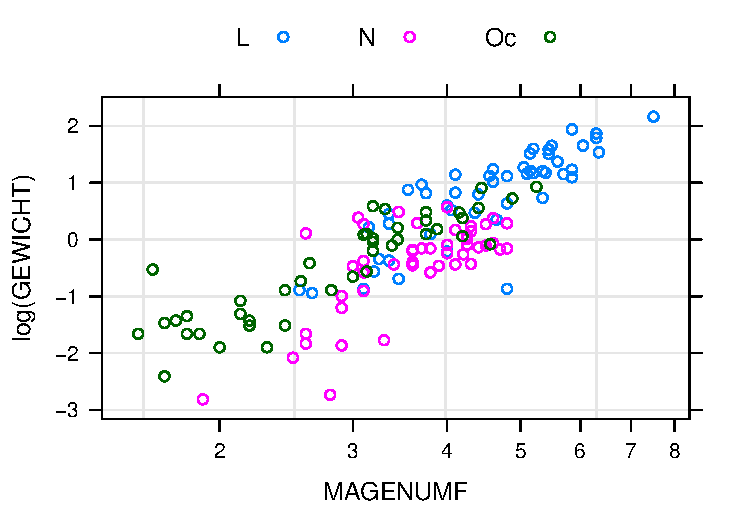
\includegraphics{Bio144_2017_week3-wurmP3}
\end{center}
}

\frame[containsverbatim]{\frametitle{}
Formulate a model (in short notation) \\[2mm]
\texttt{log(Gewicht)} $\sim$ \texttt{Magenumfang + Gattung}. \\[2mm]
Fitting it is simple in R: 

\begin{Schunk}
\begin{Sinput}
> r.lm <- lm(log(GEWICHT) ~  MAGENUMF + Gattung,d.wurm)
\end{Sinput}
\end{Schunk}
{\bf\scriptsize But make sure that Gattung is stored as a factor in R (check by \texttt{str(d.wurm)})!}
~\\[2mm]
This leads to
% latex table generated in R 3.3.1 by xtable 1.8-2 package
% Thu Oct 27 11:12:00 2016
\begin{table}[!h]
\centering
\begingroup\footnotesize
\begin{tabular}{rrrr}
  \hline
 & Coefficent & 95\%-confidence interval & $p$-value \\ 
  \hline
Intercept & -2.54 & from -2.97 to -2.10 & $<$ 0.0001 \\ 
  MAGENUMF & 0.71 & from 0.62 to 0.80 & $<$ 0.0001 \\ 
  GattungN & -0.52 & from -0.73 to -0.30 & $<$ 0.0001 \\ 
  GattungOc & -0.091 & from -0.34 to 0.16 & 0.48 \\ 
   \hline
\end{tabular}
\endgroup
\end{table}
~\\[2mm]
Why is Gattung Lumbricus (L) not in the results table? \\
Answer: L was chosen as the ``reference category'', thus $\beta_L=0$.\\[4mm]

{\bf Important:} The $p$-values of the worm species are not very meaningful. They belong to tests that compare the actual level with the reference level. However, the question is whether the species variable has an effect in total.
}

\frame[containsverbatim]{\frametitle{F-test to compare models}
\vspace{-5mm}
When a factor covariate with $k$ levels is in the model, it occupies $k-1$ parameters. Therefore, the $t$-test needs to be replaced by the $F$-test:\\[2mm]

\includegraphics[width=11cm]{pictures/Ftest.pdf}
{\small Remember: $F_{1,n-p} = t^2_{n-p}$}
}



\frame[containsverbatim]{\frametitle{F-test for the earthworms}

There exists a function (ANOVA) in R that does the $F$-test for categorical variables:\\[6mm]

\begin{Schunk}
\begin{Sinput}
> anova(r.lm)
\end{Sinput}
\begin{Soutput}
Analysis of Variance Table

Response: log(GEWICHT)
           Df  Sum Sq Mean Sq F value    Pr(>F)    
MAGENUMF    1 104.866 104.866  409.69 < 2.2e-16 ***
Gattung     2   7.177   3.589   14.02 2.842e-06 ***
Residuals 139  35.579   0.256                      
---
Signif. codes:  0 ‘***’ 0.001 ‘**’ 0.01 ‘*’ 0.05 ‘.’ 0.1 ‘ ’ 1
\end{Soutput}
\end{Schunk}

~\\[4mm]
Thus: there seems to be some difference in the regression models for the three species.
}

\frame[containsverbatim]{\frametitle{Plotting the earthworms results}
All species have the same slope (this is a modelling assumption), but different intercepts:
\begin{center}
\setkeys{Gin}{width=0.7\textwidth}
\includegraphics{Bio144_2017_week3-036}
\end{center}
}

\frame[containsverbatim]{\frametitle{Again: checking modelling assumptions}

\setkeys{Gin}{width=0.8\textwidth}
\includegraphics{Bio144_2017_week3-037}
}


\frame{\frametitle{Summary} Todo}
%\frame{References:
%\bibliographystyle{Chicago}
%\bibliography{refs}
%}

\end{document}
